\chapter{Verwaltung der Erkennungsregeln}
\label{verwaltung}

Eine Sammlung von Erkennungsregeln werden in einer Regelbasis zusammengefasst und verwaltet. Eine
Regelbasis kann aus beliebig vielen Erkennungsregeln bestehen, gehört aber immer nur zu einem
Dokumenttyp. Der Dokumenttyp gibt das Metamodell an, für welches eine Erkennungsregel bzw.
Regelbasis entwickelt wurde.

\begin{figure}[htb]
  \centering 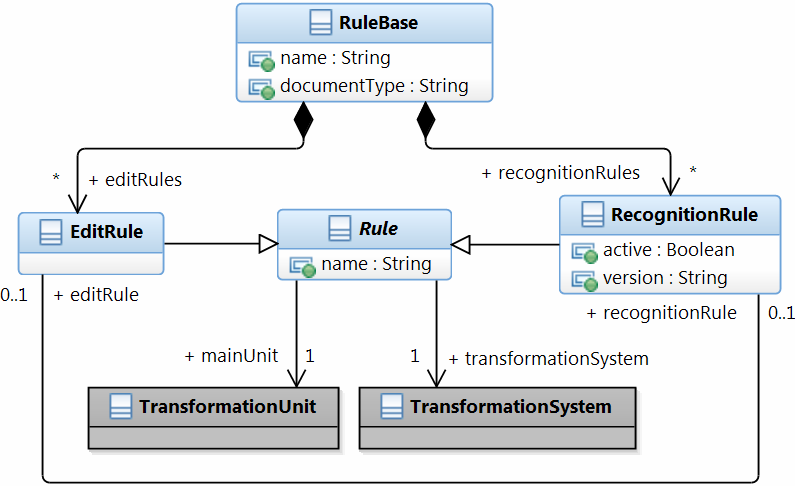
\includegraphics[scale=0.6]{images/rulebase_metamodel.png}
  \caption{Regelbasis Metamodell}
  \label{fig:rulbase_metamodel}
\end{figure}

Die Datenverwaltung wurde in Ecore modelliert. Das hat den Vorteil, dass direkte Referenzen auf die
Henshin Transformationssysteme abspeichert werden können, da diese ebenfalls auf Ecore basieren.
Neben den Erkennungsregeln können auch die entsprechend dazugehörigen Editierregel abgespeichert werden. Dies
hat den Vorteil, dass bei nachträglichen Änderungen an einer Editierregel die entsprechende
Erkennungsregel einfach erneut generiert werden kann. Sowohl die Editierregeln als auch die
Erkennungsregeln haben Namen, die später zur Anzeige und Beschreibung in der GUI dienen. Es hat sich
während der Entwicklung außerdem als nützlich erwiesen, für einzelne Test Szenarien nur bestimmte
Erkennungsregeln zu betrachten. Zu diesem Zweck können die Regeln einzeln aktiviert und deaktiviert
werden. Eine deaktivierte Regel wird später nicht auf die Differenz angewendet. Der Erkennungsregel
Generator besitzt außerdem eine Versionsnummer die bei Änderungen am Generator vom Entwickler erhöht
werden kann. Die aktuelle Versionsnummer wird dann beim Generieren in jeder Erkennungsregeln
abgespeichert. Auf diese Weise können Änderungen am Algorithmus mit den Regelbasen synchronisiert
werden.

Das vorgestellte Ecore-Modell dient ausschließlich der Datenverwaltung. Grundsätzlich ist diese
Ebene vollständig austauschbar. Die eigentliche Schnittstelle von der Regelbasis zur
Applikationslogik wird über einen s.g. Extension Point definiert.

\begin{figure}[htb]
  \centering 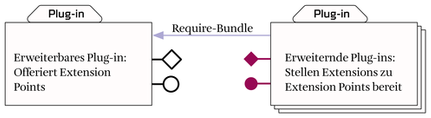
\includegraphics[scale=0.8]{images/extension_point.png}
  \caption{Extension Point \cite{ERCP2011}}
  \label{fig:extension_point}
\end{figure}

Ein Extension Point ist ein Mechanismus, mit dem Plugins unter Eclipse Schnittstellen bereitstellen
können, über die andere Plugins Erweiterungen (Extensions) anbieten können. Ein Plugin, welches eine
Erweiterung anbieten möchte, registriert dann das Schema des Extension Points in der
\textit{Extension Registry} der Eclipse-Plattform. Von dort kann das Plugin, welches den Extension
Point bereit stellt, alle Angebote nach Bedarf auslesen. \cite{ERCP2011}

Am Extension Point werden alle benötigten Informationen an die Semantic-Lifting-Engine übergeben:
Der Name und Dokumenttyp der Regelbasis sowie alle Erkennungsregeln, die auf die Differenz angewandt
werden sollen. D.h. alle Regeln, die nicht aktiviert sind müssen beim Laden direkt ausgefiltert
werden.

Um die Regelbasen möglichst komfortabel verwalten zu können, wird dem Benutzer eine auf diese
Aufgabe ausgelegte GUI zur Verfügung gestellt. Wie in Abbildung \ref{fig:rulbase_gui} zu sehen,
wird hier der Inhalt der Regelbasis als Liste angezeigt. Außerdem werden Funktionen geboten, um
diese zu ergänzen und zu verwalten.

\begin{figure}[htb]
  \centering 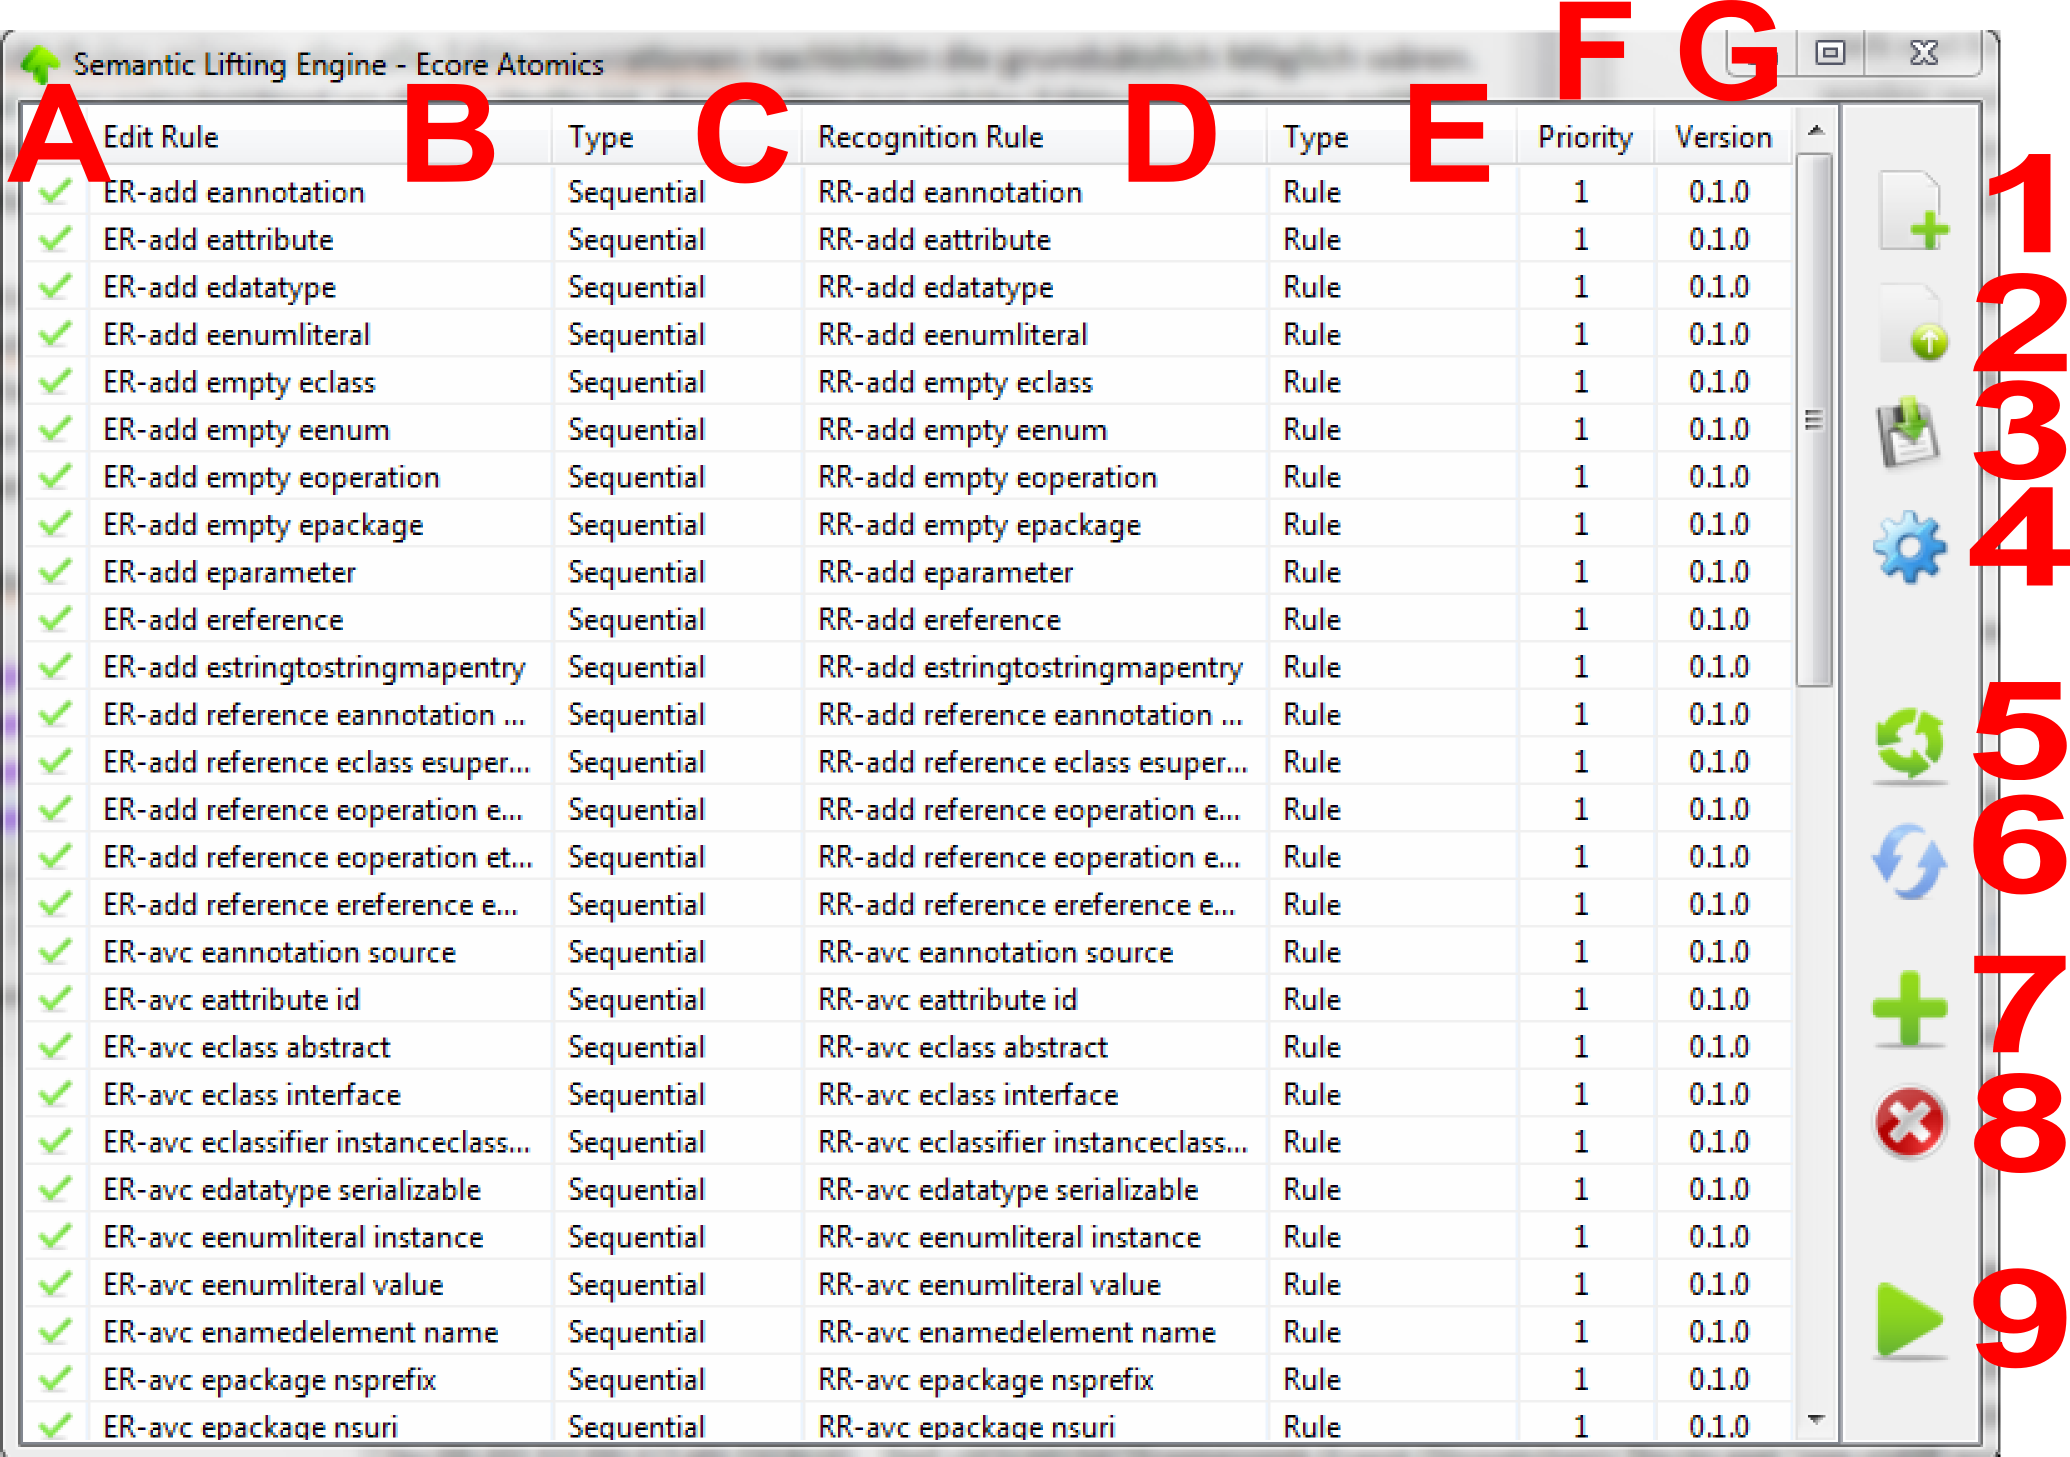
\includegraphics[width=1.0\textwidth]{images/rulebase_manager.png}
  \caption{Regelbasis Verwaltung}
  \label{fig:rulbase_gui}
\end{figure}

\begin{itemize}
  \item[\textbf{1:}] Erstellen einer neuen Regelbasis.
  \item[\textbf{2:}] Laden einer Regelbasis im XMI Format. (*.rb.xmi)
  \item[\textbf{3:}] Speichern einer Regelbasis im XMI Format. (*.rb.xmi)
  \item[\textbf{4:}] Konfigurierung der Regelbasis.
  \item[\textbf{5:}] Hier wird ein Dialog gestartet, mit dem aus einer bzw. mehreren Editierregeln
  die entsprechenden Erkennungsregeln generiert werden. Diese werden dann als neue Einträge in die
  Regelbasis eingefügt.
  \item[\textbf{6:}] Generiert die in der Liste ausgewählten Erkennungsregeln erneut.
  \item[\textbf{7:}] Startet einen Dialog, über den bereits generierte Regeln in die Regelnbasis
  aufgenommen werden können.
  \item[\textbf{8:}] Entfernt die markierten Regeln aus der Regelbasis.
  \item[\textbf{9:}] Startet den Dialog der Recognition-Engine, mit der die gesamte
  Differenz-Pipline gesteuert wird.
  \item[\textbf{A:}] Aktivieren und Deaktivieren der Erkennungsregeln für die Recognition-Engine.
  Mit einem Klick auf den Kopf der Spalte wird die Aktivierung der Regeln invertiert.
  \item[\textbf{B:}] Verwaltungsname der Editierregl. Kann editiert werden, wird aber nur zur
  Anzeige in der GUI verwendet.
  \item[\textbf{C:}] Henshin Typ der Editierregel \textit{mainUnit}.
  \item[\textbf{D:}] Verwaltungsname der Erkennungsregel. Kann editiert werden, wird aber nur zur
  Anzeige in der GUI verwendet.
  \item[\textbf{E:}] Henshin Typ der Erkennungsregel \textit{mainUnit}.
  \item[\textbf{F:}] Priorität der Erkennungsregel. (siehe \ref{post_processing} Post-Processing)
  \item[\textbf{G:}] Version des verwendeten Erkennungsregel Generators.
\end{itemize}

\begin{figure}[htb]
  \centering 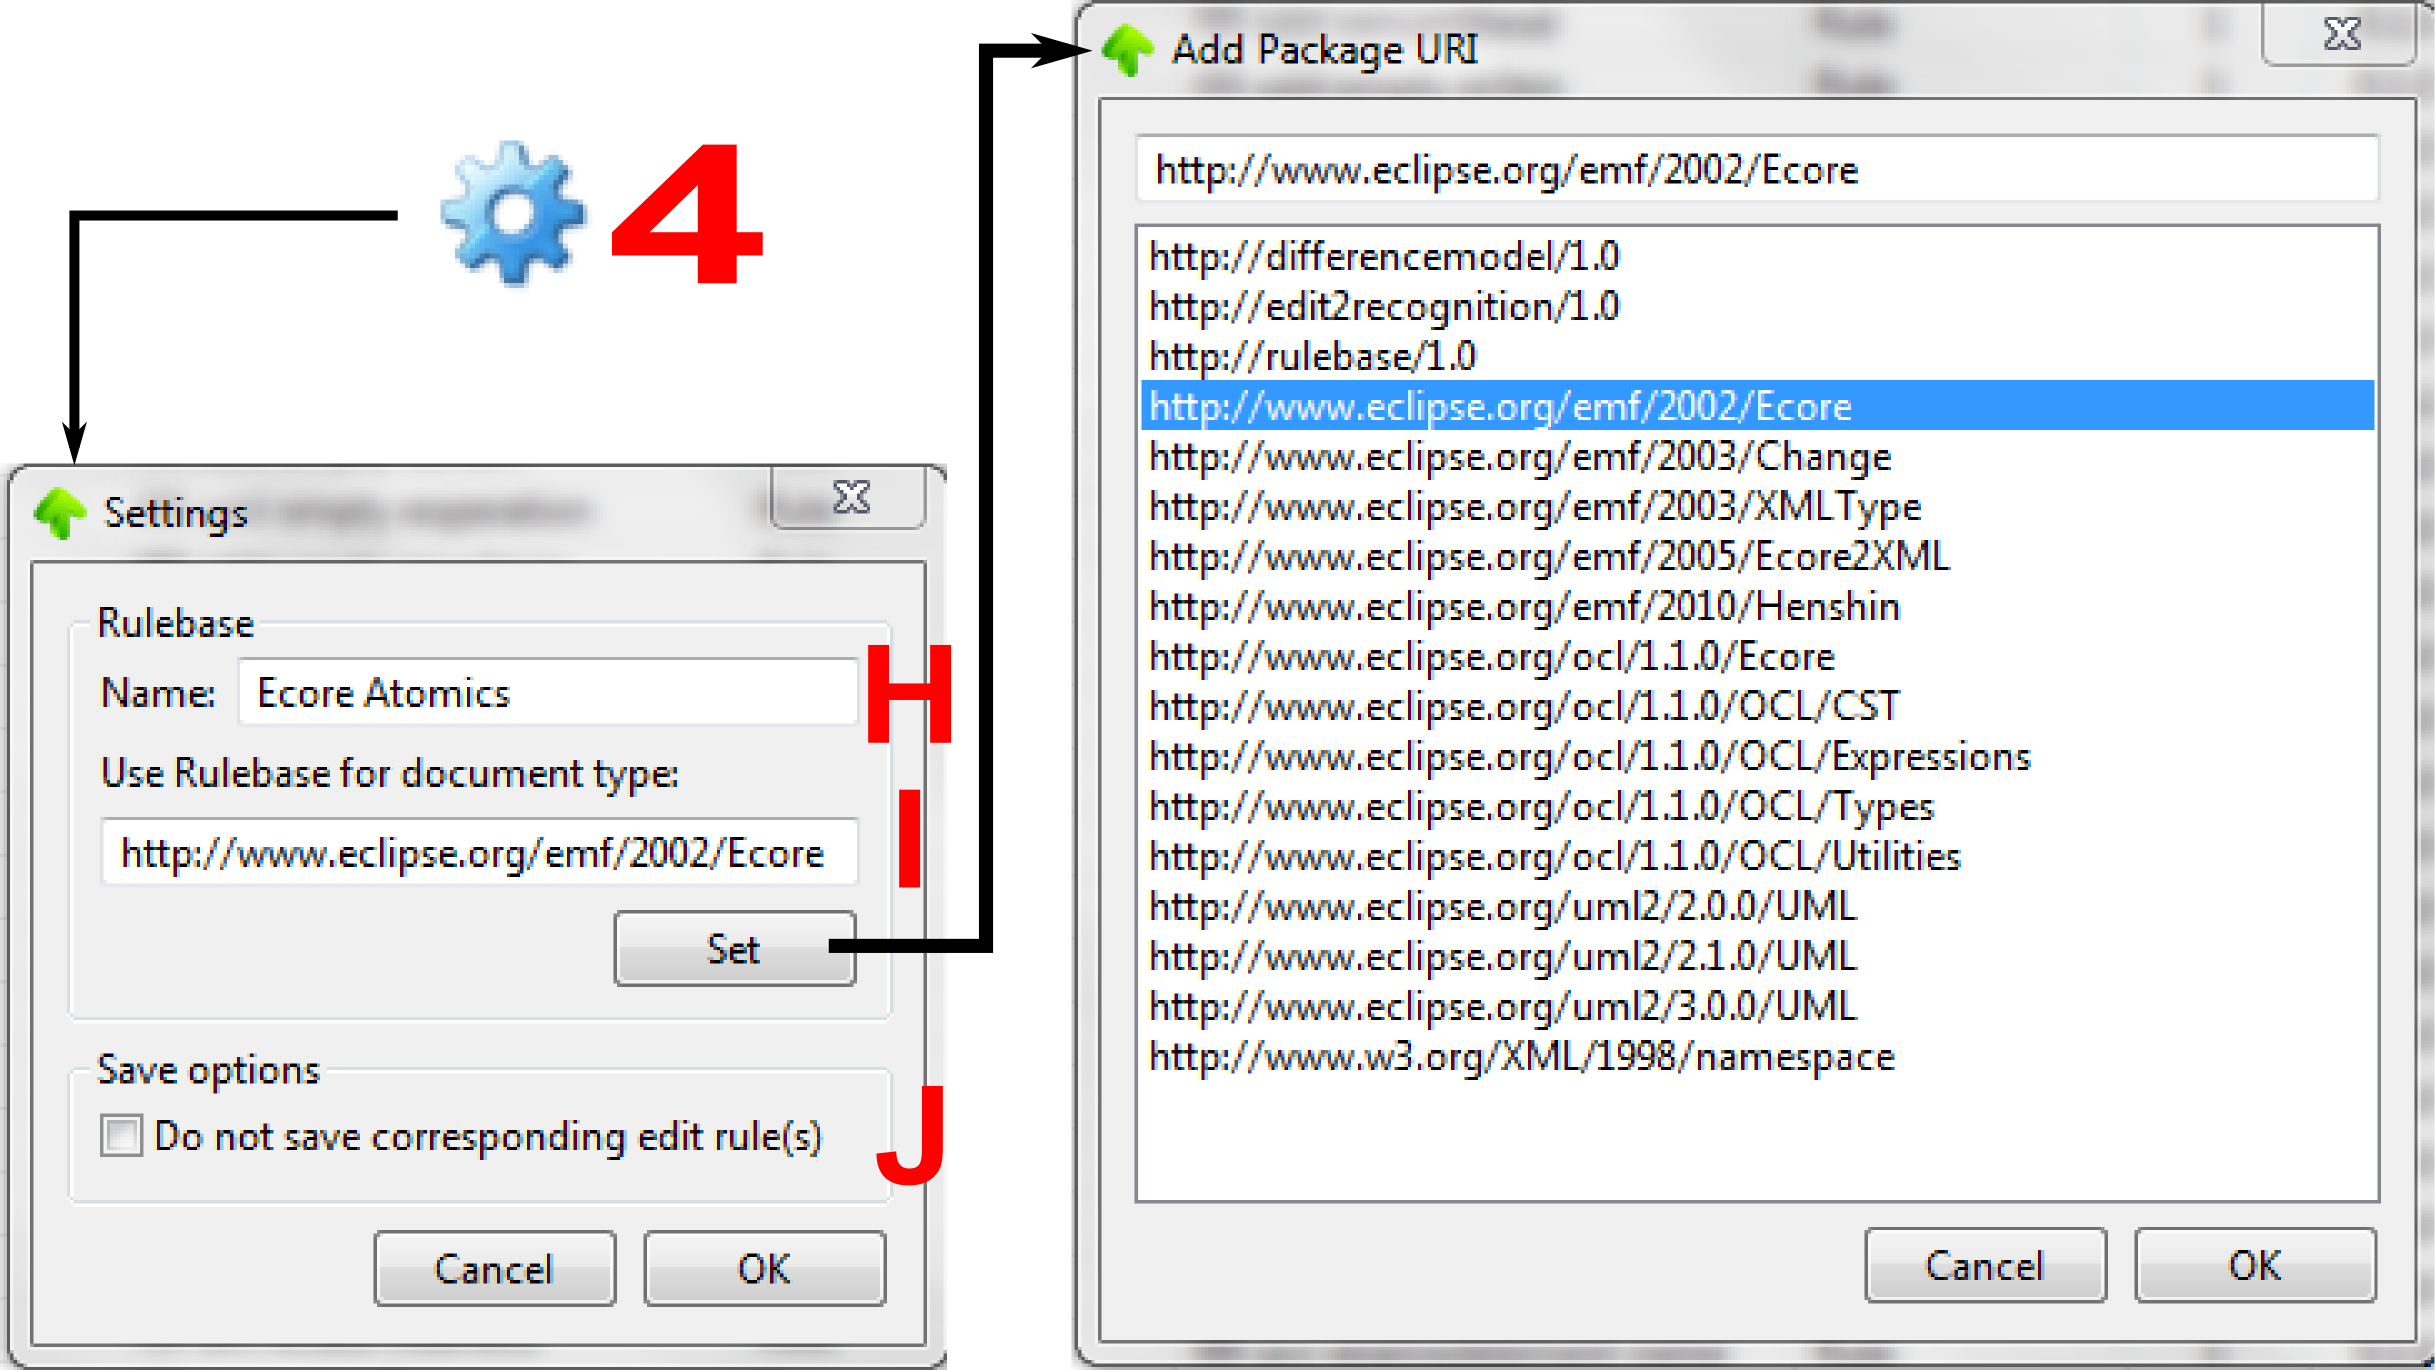
\includegraphics[scale=0.6]{images/rulebase_config_dia.png}
  \caption{Regelbasis Verwaltung - Konfiguration}
  \label{fig:rulbase_gui_config}
\end{figure}

\begin{itemize}
  \item[\textbf{H:}] Hier kann der Name der Regelbasis angegeben werden, der später in der
  Recog"-nition-Engine angezeigt wird.
  \item[\textbf{I:}] Hier wird der Dokumenttyp der Regelbasis angegeben bzw. ausgewählt. Meistens
  lässt sich der Dokumenttyp aber automatisch über die Editierregeln auslesen.
  \item[\textbf{J:}] Bei Bedarf kann hier die Verknüpfung zwischen Editier- und Erkennungsregel
  aufgelöst werden, sodass nur die Referenzen auf die Erkennungsregeln abgespeichert werden.
\end{itemize}

